\section{Modelo AS-IS}

\subsection{Modelos dos processos}
Nessa seção vamos abordar a modelagem dos processos identificados no contexto,
os processos aqui mostrados usam a notação do BPMN para dar clareza e objetividade.
Proporcionando um padrão internacional de leitura dos mesmos.

\subsubsection{Gerência de requisição}
\begin{figure}[!h]
\caption{Gerencia de requisição}
\centering % para centralizarmos a figura
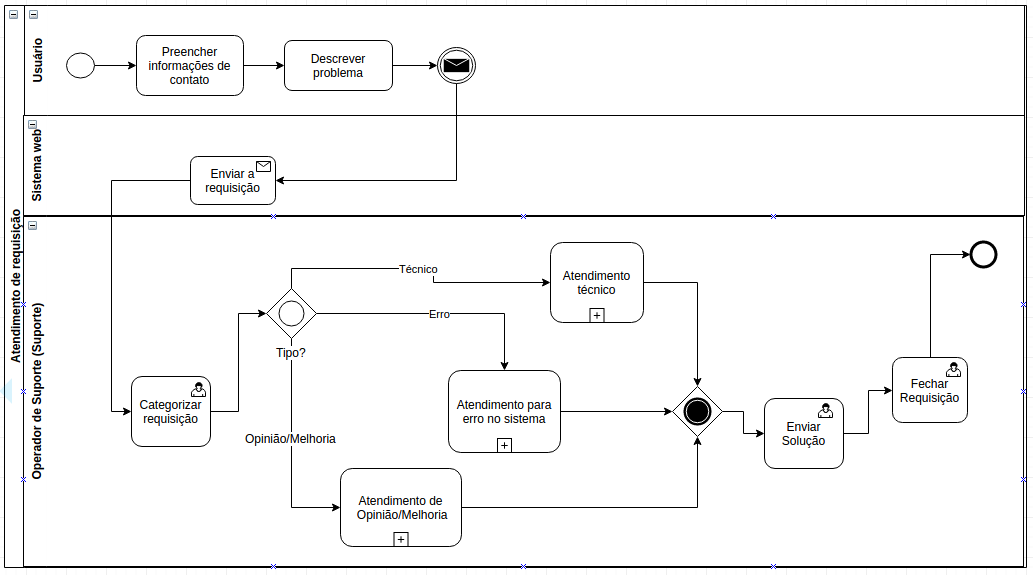
\includegraphics[width=15cm]{as-is/01_atendimento_de_requisicao.png}
\label{figura:atendimento_requisicao_as_is}
\end{figure}

\begin{itemize}[noitemsep]
	\item Preencher informações de contato
	\item Descrever problema
	\item Enviar requisição
	\item Enviar requisição
	\item Categorizar requisição
	\item Enviar Solicitação
	\item Fechar requisição
\end{itemize}

\subsubsection{Atendimento técnico}

\begin{figure}[!h]
\caption{Atendimento técnico}
\centering % para centralizarmos a figura
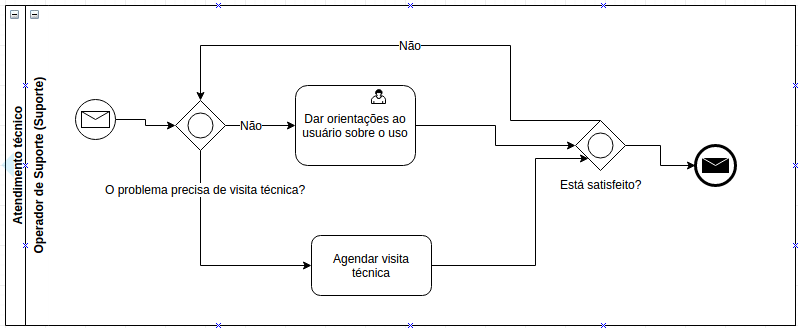
\includegraphics[width=15cm]{as-is/02_atendimento_tecnico.png}
\label{figura:suporte_tecnico_as_is}
\end{figure}

\subsubsection{Atendimento para erro no sistema}

\begin{figure}[!h]
\caption{Atendimento para erro no sistema}
\centering % para centralizarmos a figura
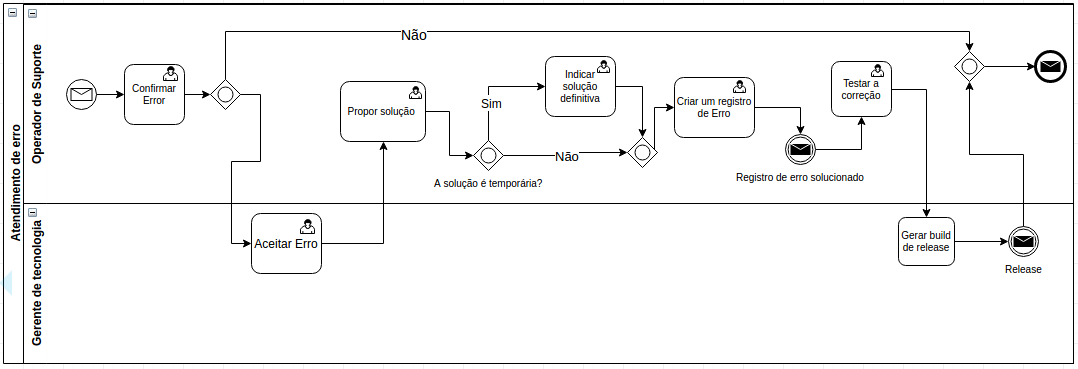
\includegraphics[width=16cm, height=5cm]{as-is/03_atendimento_de_erro.png}
\label{figura:atendimento_de_erro_as_is}
\end{figure}
\begin{itemize}
	\item Confirmar erro
	\item Aceitar Erro
	\item Propor Solução
	\item Indicar Solução definitiva
	\item Criar registro
\end{itemize}

\subsubsection{Atendimento de Opinião/Melhoria}

\begin{figure}[!h]
\caption{Atendimento de Opinião/Melhoria}
\centering % para centralizarmos a figura
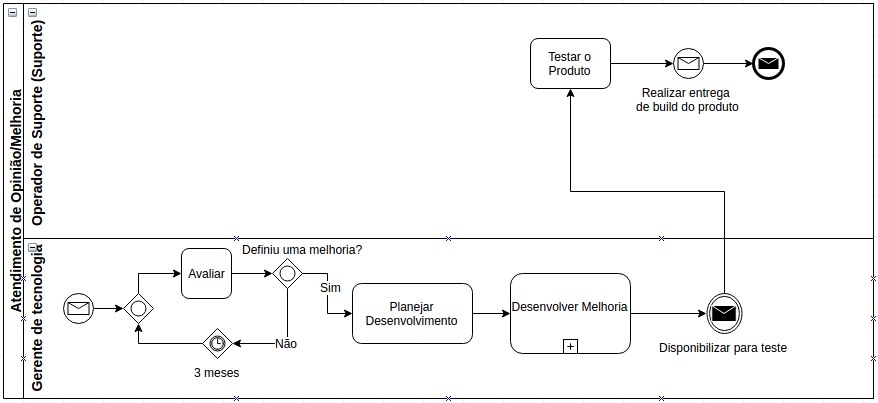
\includegraphics[width=15cm]{as-is/04_atendimento_de_melhoria.png}
\label{figura:atendimento_de_melhoria_as_is}
\end{figure}

\subsection{Conclusão e análise}
\begin{itemize}[noitemsep]
  \item Processos indefinidos
  \item Ausencia de monitoramentos
  \item Ausencia de uma base de conhecimento
  \item Ausencia de autenticação de usuário
  \item Processos de longo tempo de execução
  \item Reporte insuficiênte para o cliente
\end{itemize}
